\documentclass[11pt]{article}
\usepackage{graphicx}
\usepackage[utf8]{inputenc}
\usepackage{geometry}
\usepackage{titlesec}
\usepackage{enumitem}
\usepackage{hyperref} 
\usepackage{amsmath}
\usepackage{ gensymb }
\usepackage{ amssymb }
% \usepackage{parskip}
\usepackage{float}
\usepackage{amsthm}
\usepackage{tikz}
\usepackage{float}
\usepackage[colorinlistoftodos]{todonotes}

\setlength{\parindent}{0pt}

\theoremstyle{definition}
\newtheorem{definition}{Definition}[section]
\newtheorem{remark}{Remark}[section]

\newcommand{\R}{\mathbb{R}}
\newcommand{\N}{\mathbb{N}}
\newcommand{\Q}{\mathbb{Q}}
\newcommand{\Z}{\mathbff{Z}}
\newcommand{\st}{\text{s.t}}

\title{STAT 24310 Notes}
\author{Anthony Yoon}
\begin{document}
\maketitle
\tableofcontents
\begin{abstract}
  Notes for STAT24310 taught by Professor Yuehaw Khoo. Prior Linear Algebra knowledge will be assumed. 
\end{abstract}
\newpage
\section{Lecture 1: Introduction}
This class is heavily based on \href{https://www.stat.uchicago.edu/~lekheng/courses/309/books/Trefethen-Bau.pdf}{Trefethen and Bau's Textbook}. Take a look at it if you have the time. \\
When we run an algorithm, we often are interested in how long it takes to run the algorithm. For example, if we have a matrix $A \in \R^{n \times n}$ an $x, b \in \R^n$, and we are interested in solving 
\[
Ax = b
\]
and $n$ is very large, say $ n = 100,000$, a concern is that the algorithm takes forever to run. In this case, we may be worried about the worst case time complexity, denoted as \emph{big O notation}. In this case, solving $x = A^{-1} b$ is $\mathcal{O}(n^3)$. But what is this notation? 
\begin{definition}
  If there exists a $C \in \R$ such that for $f g$, where $g \geq 0$, where for all sufficiently $t$ large enough, such that $|f(t)| \leq C \cdot g(t)$, then $f(t) \mathcal{O}(g(t))$ 
\end{definition}
or equivantly:
\begin{definition}
  If there exists a constant \( C \in \mathbb{R} \) and a real number \( t_0 \) such that for all \( t \geq t_0 \), \( |f(t)| \leq C \cdot g(t) \), where \( g(t) \geq 0 \), then we write \( f(t) = \mathcal{O}(g(t)) \) as \( t \to \infty \).
\end{definition}
Both are equivalent. 
\section{Lecture 9: Introduction to Optimization}
Last class, we showed that there existed a solution to the Least Squares problem, or rather $\min \|Ax - b\|^2_2$ through a combination of the QR and LU decomposition. We can consider the following general optimization problem, where we define $f: \Omega \to \R$:
\[
x^* = \arg \min_{x \in \Omega} f(x)
\]
where we say that $\Omega$ is the objective domain. The intuition is that we want to find the input that would minimize the value of the function. 
\subsection{Examples}
Consider the nonlinear inverse problem used within physics. \todo{Explain this better}
\subsection{Classes of Optimization Problems}
Given a domain $\Omega$ that we want to optimize over, we have the following scenarios:
\begin{itemize}
  \item a set of discrete points, which is discrete optimization
  \item $\Omega \subseteq \R^n, \subseteq \R^n$, a constrained optimization problem. An example of this would be induced norms. 
  \item $\Omega = \R^n$, a unconstrained optimization problem. An example of this would be the Least Squares Regression Problem. 
\end{itemize}
We can often times utilize properties of the function, which is where we can introduce the idea of convexity. 
\begin{definition}
  $f$ is convex over $S$ if for any $x_1, x_2 \in S$ and $t \in [0,1]$, $f(tx_1 + (1-t)x_2) \leq tf(x_1) + (1-t)f(x_2)$
\end{definition}
This concept can be illustrated in the following diagram:
\begin{center}
  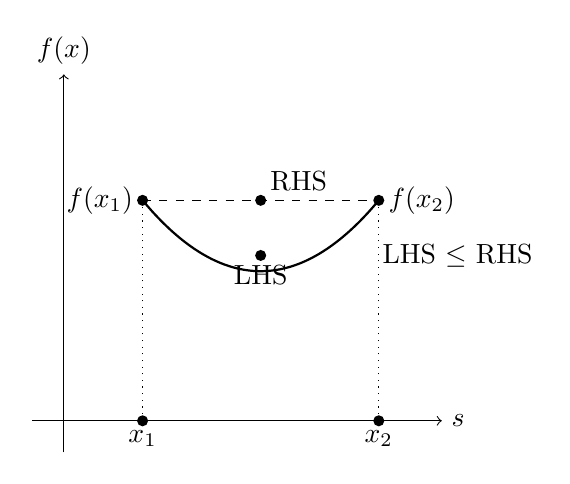
\begin{tikzpicture}[scale=2]
    % Axes
    \draw[->] (-0.2,0) -- (2.4,0) node[right] {$s$};
    \draw[->] (0,-0.2) -- (0,2.2) node[above] {$f(x)$};
  
    % Points on the x-axis
    \coordinate (X1) at (0.5,0);
    \coordinate (X2) at (2,0);
    \fill (X1) circle (1pt) node[below] {$x_1$};
    \fill (X2) circle (1pt) node[below] {$x_2$};
  
    % Function curve (convex parabola)
    \draw[domain=0.5:2,smooth,variable=\x,thick] plot ({\x},{0.8*(\x - 0.5)*(\x - 2) + 1.4});
  
    % Points on the function
    \coordinate (FX1) at (0.5,1.4);
    \coordinate (FX2) at (2,1.4);
    \fill (FX1) circle (1pt) node[left] {$f(x_1)$};
    \fill (FX2) circle (1pt) node[right] {$f(x_2)$};
  
    % RHS (linear interpolation)
    \draw[dashed] (FX1) -- (FX2);
  
    % Point on RHS (midpoint of the segment)
    \coordinate (RHS) at (1.25,1.4);
    \fill (RHS) circle (1pt);
    \node[above right] at (RHS) {RHS};
  
    % LHS point (on the function)
    \coordinate (LHS) at (1.25,1.05);
    \fill (LHS) circle (1pt);
    \node[below] at (LHS) {LHS};
  
    % Dashed lines from x1 and x2 to function
    \draw[dotted] (X1) -- (FX1);
    \draw[dotted] (X2) -- (FX2);
  
    % Inequality annotation
    \node at (2.5,1.05) {LHS $\leq$ RHS};
  
  \end{tikzpicture}
\end{center}
We can then expand the definition of convexity as follows:
\begin{definition}
    $f$ is strongly convex over $S$ if for any $x_1, x_2 \in S$ and $t \in [0,1]$, $f(tx_1 + (1-t)x_2) < tf(x_1) + (1-t)f(x_2)$
\end{definition}
A natural expansion of this is when $f$ is convex, then $f \left( \sum_{i = 1}^{n} t_i x_i \right) \leq \sum_{i = 1}^{n} t_i f(x_i)$ where $\sum_{i = 1}^{n} t_i = 1$ such that $t_i \geq 0$. We can also consider the following definition of convexity:
\begin{definition}
  Locally Convex: $f: \Omega \to \R$, where $f$ is convex over some $S \subseteq \Omega$
\end{definition}
\subsection{Taylor's Theorem}
We begin with an introduction of smoothness.
\begin{definition}
  A function is said to be $C^n$ if it is contionus and differentiable $n$ number of times. 
\end{definition}
Also a refresher on what the Taylor's Theorem in 1D is. 
\begin{definition}
  if $f: \R \to \R$ is $(k+1)$ times differentiable at $x = a$, then 
  \[
  f(x) = f(a) + \frac{\partial f(a)}{\partial x}(x-a) + \dots + \frac{1}{k!} \frac{\partial^k f(x)}{\partial x^k}(x-a)^k + \frac{L}{(k+1)!}(x-a)^{k+1}
  \]
  where 
  \[
  L = \sup_{\xi \in [x,a]} \left| \frac{\partial^{k+1} f(x)}{\partial x^k} \right|
  \]
\end{definition}
note that if $|x-a|$ is sufficiently small, we can discard the remainder the term (the one with the $L$ in it). Note that also that if the $(k+1)$ derivative is bounded, then we can approximate $f$ with the kth order polynomial. We can also consider the case of the special case of the third order taylor polynomial expansion. 
\begin{definition}
  For $f: \R^n \to \R$, and $f$ has a bounded 3rd deriative, the expansion is as follows
  \[
  f(x) = f(a) + \frac{\partial f(a)}{\partial x} (x-a) + \frac{1}{2}(x-a^T) H(a)(x-a) + \mathcal{O}(\|x-a\|^3)
  \]
  where we define
  \[
  H(a)_{ij} = \frac{\partial f(a)}{\partial x_i \partial x_j}
  \]
  where $H(a)$ is $n \times n$
\end{definition}
To illustrate the nature of the Hessian Matrix, we can visualize $f$ locally to see that we can use a contour map. The Hessian usually shows the directions of the biggest changes in direction, given by the Eigenvalues. \todo{Need to fix}


However, we can see that if our function is convex and smooth, then \emph{optimality is guarantted based on the local deriative}. We can see this in the following proof:
\begin{proof}
  if $f$ is convex and differentiable, we can see that if we let $a,b$ be in the domain of $f$. we can see that we are left with the following inequality. 
  \[
  f(b) \geq f(a) + \frac{\partial f(a)}{\partial x}(b-a)
  \]
  by the definition of convexity. If we choose $a$ such that $f'(a) = 0$, we see that we have guarnteed an optimal solution. 
\end{proof}
However, we can see that if we are working with a strongly convex differentiable solution, we can use the same assumptions as above to see in the following proof. 
\begin{proof}
  We are given that $f$ is strongly convex and differentiable. Thus, we can see that for the following taylor expansions 
  \[
  f(b) \geq f(a) + \frac{\partial f(a)}{\partial x}(b-a) + \frac{a}{2} \|b - a\|_2^2
  \]
  We see that we can choose a point such that $\frac{\partial f(a)}{\partial x} = 0$, which implies that 
  \begin{align*}
    f(b) &\geq f(a) + \frac{a}{2} \|b - a\|^2\\
    \implies  & f(b)  > f(a), \forall b, b \neq a
  \end{align*}
  Since we know that the function is strongly convex and thus, we know that for any point $b$ and $a$. the last inequality holds, we can see that we have indeed foound the unique optimizer.
\end{proof}
\begin{remark}
  Strongly convex implies strictly convex, but not the other way around. 
\end{remark}
\subsection{Applications of convexity}
Consider the following:
\[
f(x) = \frac{1}{2} ax^2 - bx, a > 0
\]
and consider the following:
\begin{align*}
  f(x) &= \frac{1}{2}ax^2 - bx\\
  f(y) - f(x) &= \frac{1}{2}a(y^2 - x^2) - b(y-x)
\end{align*}


\end{document}